\documentclass[]{book}
\usepackage{lmodern}
\usepackage{amssymb,amsmath}
\usepackage{ifxetex,ifluatex}
\usepackage{fixltx2e} % provides \textsubscript
\ifnum 0\ifxetex 1\fi\ifluatex 1\fi=0 % if pdftex
  \usepackage[T1]{fontenc}
  \usepackage[utf8]{inputenc}
\else % if luatex or xelatex
  \ifxetex
    \usepackage{mathspec}
  \else
    \usepackage{fontspec}
  \fi
  \defaultfontfeatures{Ligatures=TeX,Scale=MatchLowercase}
\fi
% use upquote if available, for straight quotes in verbatim environments
\IfFileExists{upquote.sty}{\usepackage{upquote}}{}
% use microtype if available
\IfFileExists{microtype.sty}{%
\usepackage{microtype}
\UseMicrotypeSet[protrusion]{basicmath} % disable protrusion for tt fonts
}{}
\usepackage[unicode=true]{hyperref}
\hypersetup{
            pdftitle={A First Course in Probability and Statistics},
            pdfauthor={Nick Syring},
            pdfborder={0 0 0},
            breaklinks=true}
\urlstyle{same}  % don't use monospace font for urls
\usepackage{natbib}
\bibliographystyle{plainnat}
\usepackage{longtable,booktabs}
\usepackage{graphicx,grffile}
\makeatletter
\def\maxwidth{\ifdim\Gin@nat@width>\linewidth\linewidth\else\Gin@nat@width\fi}
\def\maxheight{\ifdim\Gin@nat@height>\textheight\textheight\else\Gin@nat@height\fi}
\makeatother
% Scale images if necessary, so that they will not overflow the page
% margins by default, and it is still possible to overwrite the defaults
% using explicit options in \includegraphics[width, height, ...]{}
\setkeys{Gin}{width=\maxwidth,height=\maxheight,keepaspectratio}
\IfFileExists{parskip.sty}{%
\usepackage{parskip}
}{% else
\setlength{\parindent}{0pt}
\setlength{\parskip}{6pt plus 2pt minus 1pt}
}
\setlength{\emergencystretch}{3em}  % prevent overfull lines
\providecommand{\tightlist}{%
  \setlength{\itemsep}{0pt}\setlength{\parskip}{0pt}}
\setcounter{secnumdepth}{5}
% Redefines (sub)paragraphs to behave more like sections
\ifx\paragraph\undefined\else
\let\oldparagraph\paragraph
\renewcommand{\paragraph}[1]{\oldparagraph{#1}\mbox{}}
\fi
\ifx\subparagraph\undefined\else
\let\oldsubparagraph\subparagraph
\renewcommand{\subparagraph}[1]{\oldsubparagraph{#1}\mbox{}}
\fi
\usepackage{booktabs}

\title{A First Course in Probability and Statistics}
\author{Nick Syring}
\date{2022-01-24}

\begin{document}
\maketitle

{
\setcounter{tocdepth}{1}
\tableofcontents
}
\chapter{About}\label{about}

This is a collection of notes intended for students studying probability
and statistics at the advanced undergraduate level at Iowa State
University. Specifically, these notes are modeled after course notes for
STAT 588, 341, and 342. This site is a work in progress.

Some relevant textbook references include John E. Freund's Mathematical
Statistics with Applications by Miller and Miller, although many books
on this material are available.

\chapter{Experiments and the role of
probability}\label{experiments-and-the-role-of-probability}

In this chapter we introduce concepts related to scientific studies,
data collection, and random sampling.

\section{Experiments}\label{experiments}

There are many settings in which data is collected and studied. In this
course we will limit our focus to \emph{random sampling experiments} and
\emph{random sampling, randomized intervention experiments} defined
below.

Both of these settings start with a \emph{research question} of interest
in the the context of a \emph{population} or set of individuals. For
example, in a political poll the population is the set of eligible
voters and the research question is ``which of two candidates has
majority support?''

Experiments like polls necessarily only measure an outcome or
\emph{response} (like voter preference) for a limited number of
individuals from the population. The collection of observed individuals
is the \emph{sample}. For many reasons relating to, e.g., cost, time,
and access, the size of the sample is small compared to the size of the
population. On the other hand, there are rare instances in which a whole
population is observed, and we call this a \emph{census}. In a census,
all possible information is gathered, whereas in an experiment only a
limited subset of information is obtained. We will be concerned only
with experiments and how best to use the limited information gathered in
order to answer research questions.

When only a sample of a population is available a natural question is
``how is the sample determined?'' If there is freedom in the choice of
sample then ``how should the sample be chosen?'' Intuitively, if we can
only observe some of the individuals belonging to the population then we
prefer to observe a \emph{representative} sample of them. Representative
means that the heterogeneities/differences between individuals that
exist in the population ought to be more or less accurately reflected in
the sample. For example, a poll of eligible voters in Iowa is not
representative if it includes only registered Democrats, and we would
not expect such a poll to accurately reflect the population preference
between two candidates. If we have a representative sample from the
population then we assume the results of our experiment are
\emph{generalizable} to the population. In other words, the observations
we make are characteristic of the population and we would not expect
vastly different observations had we obtained a different, similarly
representative sample, or if we had observed the whole population. There
are different ways to obtain representative samples. One way is via
\emph{stratified sampling}. For example, suppose we knew or could
measure the relative population proportions of all factors relevant to
voting preference, say, party affiliation, sex, age, income level,
education level, and religious affiliation. Then, we could construct a
sample of individuals with values of these demographic variables
matching the levels present in the population---a representative
sample---by randomly selecting the right number of individuals from each
of these subgroupings or \emph{strata}. However, this takes a lot of
information to pull off. Instead, researchers typically attempt to
construct a \emph{simple random sample} of individuals from the
population. A simple random sample (SRS) of size \(n\) from a finite
population means every subset of \(n\) individuals is equally likely to
be chosen. You can imagine a SRS as pulling numbers out of a hat, so to
speak. An SRS of eligible voters could be constructed, for instance, by
randomly choosing 100 social security numbers from the list of SSNs of
all eligible voters. SRSs are not always trivial to construct---as in
the polling example they require a list of population individuals, which
may be difficult to obtain.\\

We are at the point where we can define a \emph{random sampling
experiment} as the process by which we select a SRS from a population
and record a response from sampled individuals for the purpose of
answering a research question. As noted, an important example is a poll.

Random sampling experiments are valuable, but limited to addressing
questions about one variable at a time. In many cases researchers are
interested in how one variable affects the value of another, and these
questions can often be answered using interventional experiments. An
\emph{intervention} is an act by a researcher intended to affect the
value of the response variable in sampled individuals. When an
intervention is applied to samples the samples are often referred to as
\emph{experimental units}. An important example of an interventional
experiment is a clinical trial. In a basic clinical trial a random
sample of patients is recruited from a population of patients with a
certain medical condition. Then, a subset of the patients is given a
treatment of interest --- the intervention --- while the other patients
are given a different treatment or perhaps no treatment at all (maybe a
placebo). The response, probably related to the health of patients
post-treatment, is then compared between the intervention and
non-intervention groups. This experiment is like a random sampling
experiment with an added intervention step. The key question is ``how do
we determine which experimental units receive the intervention?'' Recall
that when we obtain a sample of individuals from a population we wish to
do so in such a way as to obtain a representative sample. The same idea
applies to interventions. The group of samples receiving the
intervention should be similar to the group not receiving the
intervention; that is, both groups should be representative of the total
set of sampled individuals. Therefore, it makes sense to
\emph{randomize} the application of the intervention over sampled
individuals.

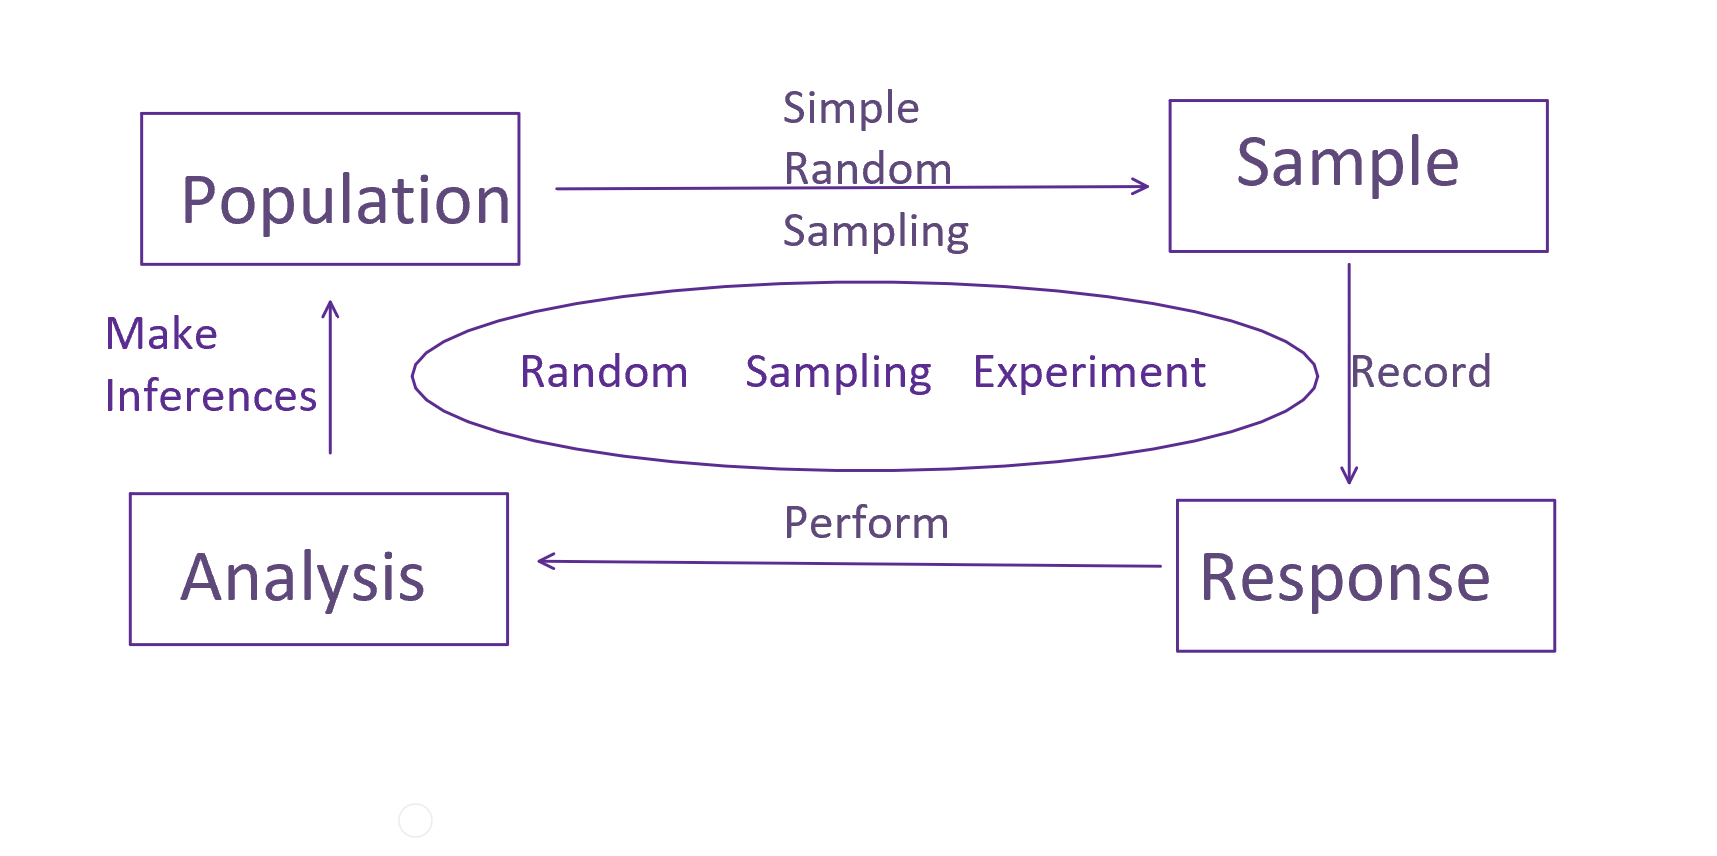
\includegraphics[width=23.85in]{rsediagram} A \emph{random sampling,
randomized intervention experiment} consists of obtaining a SRS from a
population, randomizing an intervention over those samples, and
recording a response variable relating to a research question. This type
of experiment is often explained by conceptualizing two (or more)
different populations. Suppose the experiment is a clinical trial and
the intervention consists of receiving a treatment versus no treatment.
Then, we can interpret the randomization step as defining two SRSs from
two (abstract or hypothetical) populations: a sample from the set of
treated patients and a sample from the set of untreated patients. The
research question typically concerns the relationship between these two
populations, such as, ``are treated patients, on average, healthier than
untreated patients, with respect to the response variable?''

We will only consider randomized interventional experiments. Briefly,
consider what can go wrong if we do not randomize intervention. Suppose
the patients in our clinical trial consist of both old and young people
and that old people are generally more in need of treatment. If we give
the treatment to only young(old) people, then we will
underestimate(overestimate) the effect of the treatment compared to what
its effect would be, on average, over the whole population. In effect,
we have \emph{confounded} the treatment/intervention effect with the
effect of age on the response. This may seem like a silly example
because we could easily avoid assigning the intervention to only young
or only old people. But, not all potential confounding variables are
obvious/visible. Unknown confounders, also called \emph{lurking
variables}, can only be systematically accounted for via randomizing the
intervention. Of course it is possible for randomized groups not to be
representative in a particular occurrence, but, systematically,
randomized groups will tend to be representative, so it's a good
practice.

When the intervention is randomized we cautiously assume substantial
differences in the observed responses between intervention groups can be
attributed to the intervention. In other words, we believe in
\emph{causation}---that the intervention caused the observed
differences. When confounding variables are present we never know which
variable is responsible for observed differences in responses and we
cannot support claims about cause and effect relationships using the
data alone.

In some studies researchers analyze the relationships between variables
without performing randomized interventions; these are usually
\emph{observational studies}. For instance, in the Framingham Heart
Study, researchers recorded the health and lifestyle choices of
Massachusetts residents over several years. By collecting a large amount
of data they were able to establish a strong relationship or
\emph{association} between cigarette smoking and cancer. Their data
alone is not enough to imply causation, but their study inspired many
follow-up experiments like lab experiments on animals, and the
development of biochemical theories about tumor development. The
combination of these various works leaves little doubt today that
tobacco use dramatically increases the likelihood of developing cancer.

\section{The role of probability}\label{the-role-of-probability}

Consider the example of a political poll on the preferences of voters
between two candidates---this is a random sampling experiment. The
population consists of all eligible voters in the upcoming election.
Each voter can be associated, say, with a 1 or a 0, indicating their
preference between the two candidates. Let these 0-1 preferences be
denoted \(x_1, \ldots, x_N\) where \(N\) is the population size. There
exists a population level value \(\theta\) equal to
\[\theta:=N^{-1}\sum_{j=1}^N x_j\] denoting the population voter
preference; this is the \emph{population proportion}. Most research
questions of interest concern the unknown value of \(\theta\). In the
polling experiment we observe a random subset of \(x_1, \ldots, x_N\)
values, say, \(X_1, \ldots, X_n\) for \(n<N\)---keep in mind these are
not the first \(n\) x's, but a random subset of \(n\) x's.
Correspondingly, we can compute the sample voter preference
\[\hat\theta_n := n^{-1}\sum_{i=1}^n X_i.\] For every possible sample of
\(n\) voters, there is a corresponding value of \(\hat\theta_n\). We can
think of the polling experiment as randomly choosing one of these
\(\hat\theta_n\) values out of a hat containing all of them. Randomly
sampling voters causes randomness in the observed \(\hat\theta_n\)
preference value. The mathematics of \emph{probability} is used to
quantify this randomness, e.g., to be able to compute the chance of
\(\hat\theta_n\) taking on any particular value, given knowledge of the
population.

That last phrase ``given knowledge of the population'' is very
important, and illustrates the difference between probability and
statistics (inference) quite succinctly. Probability characterizes the
chance of observing a particular random sample given the population,
whereas statistics seeks to explain some characteristic of the
unknown/unobserved population given only one sample (subset of
population individuals).

Probability plays a key role in statistics problems, and the first part
of our course is devoted to developing methods for computing
probabilities of samples in a variety of useful special cases.

Let's illustrate this interplay of probability and statistics by
continuing the example of a poll. The population, again, can be
represented by \(N\) values, each either a \(0\) or a \(1\) indicating
each voter's preferences, and we can label these \(x_1, \ldots, x_N\). A
poll is a random sample of \(n\) of these values, labeled
\(X_1, \ldots,X_n\), without replacement, i.e., once a value \(x_j\) is
selected and recorded it cannot be selected again (no double voting!).
The population preference \(\theta\) is the average of \(x_j\)'s for
\(j=1, \ldots, N\). If we knew the size of the population \(N\) and the
population proportion \(\theta\), then we could compute the chance of
observing any \(\hat\theta_n := n^{-1}\sum_{i=1}^n X_i\) value according
to the rules of probability (which we will soon study). For example, if
\(N\) is much larger than \(n = 10\) and \(\theta = 1/2\), then the
chance of observing exactly \(\hat\theta = 1/2\) is about \(25\%\) (it's
about equal to \(252\theta^5(1-\theta)^5\)). Of course, the whole point
of the poll is to learn something about the unknown value of \(\theta\),
so we cannot actually perform this probability calculation in practice.
But, consider connecting the probability calculation to our goal. We
would like to distinguish between values of \(\theta\) that are more or
less plausible. Suppose we conduct the poll of \(10\) individuals and
observe \(\hat\theta = 1/2\). Then, our probability calculation says the
probability we observe \(\hat\theta = 1/2\) is highest if
\(\theta = 1/2\). In other words, \(1/2\) is the most plausible value of
the population proportion given our observations. Intuitively, we expect
values near \(1/2\) are more plausible than values far from \(1/2\).
This correspondence between the probability calculation and plausible
values of the \emph{population parameter} is called the \emph{maximum
likelihood principle} which we will study in a later chapter.

\section{Exercises}\label{exercises}

\begin{enumerate}
\def\labelenumi{\arabic{enumi}.}
\item
  Google James Lind's Scurvy experiments. What was James' research
  question? What was the population? Did he obtain a random sample from
  the population? If not, does that make you suspicious of his findings?
  Why or why not? Did James use any interventions? If so did he
  randomize them? Do you think his randomization scheme is reliable?
  What were his conclusions?
\item
  Find a recent example of an experiment in the news or a scientific
  publication. Describe the research question, population, intervention
  (if there is one), and response. Is it a random sampling experiment, a
  random sample randomized intervention experiment, or something else,
  like an observational study?
\item
  The Challenger space shuttle exploded when it experienced o-ring
  failures thought to be caused by low launch temperature. The launch
  temperature was 31 degrees Fahrenheit. The following data can be
  interpreted as a random sample of counts of o-ring failures from a
  population of launches. Given this data do you think we can make
  reliable conclusions about launch safety at 31 degrees launch
  temperature? What concepts discussed in this section are relevant
  here?
\end{enumerate}

\begin{table}

\caption{\label{tab:unnamed-chunk-2}A table of o rings at risk, o ring failires, and launch temperatures of space shuttle flights.}
\centering
\begin{tabular}[t]{rrr}
\toprule
at risk & failed & launch temp.\\
\midrule
6 & 1 & 70\\
6 & 0 & 69\\
6 & 0 & 68\\
6 & 0 & 67\\
6 & 0 & 72\\
\addlinespace
6 & 0 & 73\\
6 & 0 & 70\\
6 & 1 & 57\\
6 & 1 & 63\\
6 & 1 & 70\\
\addlinespace
6 & 0 & 78\\
6 & 0 & 67\\
6 & 2 & 53\\
6 & 0 & 67\\
6 & 0 & 75\\
\addlinespace
6 & 0 & 70\\
6 & 0 & 81\\
6 & 0 & 76\\
6 & 0 & 79\\
6 & 0 & 75\\
\addlinespace
6 & 0 & 76\\
6 & 1 & 58\\
\bottomrule
\end{tabular}
\end{table}

\chapter{Probability and Counting}\label{probability-and-counting}

Probability is a tricky subject. We have an intuitive sense about
probability, but we use it in different ways, which can sometimes lead
to confusion. Probability is used in at least two ways: -to describe the
relative frequency of events, e.g., what is the chance of observing 5
heads in the next ten flips of a fair coin; and, -to communicate degrees
of belief, e.g., the Packers have a 30\% chance of winning the Super
Bowl.

We will use probability exclusively in the sense of the first
interpretation---to characterize the chances of different outcomes in
repeatable trials. This sense of probability corresponds to
characterizing the possible outcomes of random sampling. Although
probability is often used to communicate degrees of belief there are
good reasons not to use it for this purpose, but a formal, nuanced
discussion of quantification of beliefs is outside our present purview.

\section{Terminology}\label{terminology}

In our discussion of probability we will think of an \emph{experiment}
as the act of measuring/observing a variable on one or more random
samples from a population. The \emph{sample space} is the set of
possible realizations of the experiment. For example, if the experiment
is to flip one coin and record whether it is heads or tails, then we can
think of this as a random sampling from sample space \(\{H, T\}\) where
the outcome may be either \(\{H\}\) or \(\{T\}\). Any subset of the
sample space of an experiment is an \emph{event}; for example, \(\{H\}\)
and \(\{H,T\}\) are events, and so is \(\emptyset\) which denotes the
``empty set'', the set of nothing.

\section{Set relations}\label{set-relations}

Events and sample spaces are sets, and we will make use of relations
between sets. -Set union: for sets/events A and B, \(A\cup B\) denotes
the set of elements in at least one of \(A\) or \(B\). For example,
\(\{1,2,3\}\cup\{3,4,5\} = \{1,2,3,4,5\}\). -Set intersection:
\(A\cap B\) denotes the set of elements in both A and B. For example,
\(\{1,2,3\}\cap\{3,4,5\} = \{3\}\). -Set complement: \(A^c\) denotes the
set of elements in the sample space \(\mathcal{S}\) but not in \(A\).
For example, if \(\mathcal{S} = \{1,2,3,4,5\}\) then \(A^c = \{4,5\}\).
-Set subtraction: \(A\backslash B\) of \(A-B\) means \(A\cap B^c\) which
is the set of elements in \(A\) but not in \(B\). For example,
\(\{1,2,3\}-\{3,4,5\} = \{1,2\}\).\\

\subsection{Sample space example}\label{sample-space-example}

Here's an example to illustrate sample spaces. A gas station has six
pumps, A, B, C, D, E, F. -What is the sample space of the number of
pumps in use? \(\mathcal{S} =\{0,1,2,3,4,5,6\}\). -What is the sample
space of pumps in use?
\(\mathcal{S} = \{\{A,B,C,D,E,F\},\{A,B,C,D,E\}, \ldots,\{F\}, \emptyset \}\).
This is the \emph{power set} of \(\{A,B,C,D,E,F\}\), the set of all
subsets of those pumps. Fun fact: if the sample space \(\mathcal{S}\)
consists of \(N\) elements then its power set, written
\(2^{\mathcal{S}}\), contains \(2^N\) elements. Can you see why?
-Suppose you test pump A every day until it fails to function. What is
the sample space of this experiment?
\(\mathcal{S} = \{F, SF, SSF, \ldots \}\). This is a \emph{countably
infinite} sample space. -You measure the amount of gas pumped by the
next customer. \(\mathcal{S} = (0, ?)\), an interval with some upper
bound equal to however much gas the station has available. This is an
\emph{uncountably infinite} sample space.

\subsection{Set relations example}\label{set-relations-example}

This next example illustrates set relations.

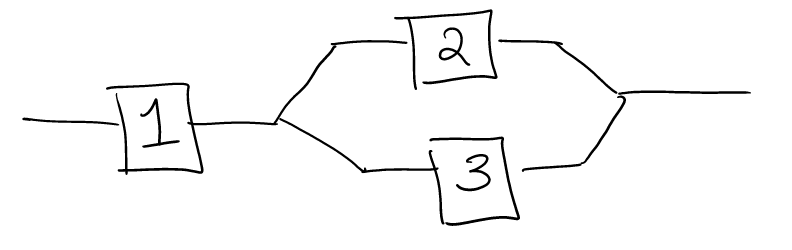
\includegraphics[width=11in]{system} Consider this system of series and
parallel components. Each component either functions/succeeds (S) or
fails (F). The experiment simply observes if the system
functions/succeeds or fails. -What is the sample space in terms of the
three components?
\(\mathcal{S} = \{SSS, SSF, SFS, FSS, SFF, FFS, FSF, FFF\}\). -Find the
even two components succeed. \(A = \{SSF, SFS, FSS\}\). -Find the even
at leas two components succeed.
\(B = \{SSF, SFS, FSS, SSS\} = A\cup \{SSS\}\). -Find the event the
system functions. \(C = \{SSS, SFS, SSF\}\).

\section{Probability Axioms}\label{probability-axioms}

Andrey Kolmogorov formalized rules/axioms of probability we are mostly,
intuitively familiar with.

\begin{enumerate}
\def\labelenumi{\arabic{enumi}.}
\tightlist
\item
  The probability of the sample space is 1, \(P(\mathcal{S})=1\).
\item
  Probabilities are non-negative. If \(A\subset\mathcal{S}\) then
  \(P(A)\geq 0\).
\item
  Countable additivity. This last one is a bit tricky. Let's start with
  an intuitive, simpler case. Suppose \(\mathcal{S} = \{1,2,3,4,5\}\).
  The important part is \(\mathcal{S}\) is finite and includes only
  different things that don't ``overlap''. Then, we know that, for
  example, \(P(\{1\}\cup \{2\}) = P(\{1\}) + P(\{2\})\), which says that
  the probability of the union of \emph{disjoint} events equals the sum
  of probabilities of each event. Kolmogorov requires this extends to
  countably infinite \(\mathcal{S}\), hence the name countable
  additivity. Specifically, let events \(A_1\), \(A_2\), \(\ldots\) be a
  sequence of mutually disjoint events (none overlap, like pizza slices)
  so that \(A_i \cap A_j = \emptyset\) for every \(i\ne j\). Then,
  \[P\left(\bigcup_{i=1}^\infty A_i\right) = \sum_{i=1}^\infty P(A_i).\]
\end{enumerate}

There are a number of important consequences of the axioms: *
Complementarity - \(P(A^c) = 1-P(A)\) * Inclusion-exclusion principle
\[P(A\cup B) = P(\{A\cap B\}\cup\{A-B\}\cup\{B-A\})\]
\[ = P(A)+P(B)-P(A\cap B)\]

\subsection{Example of using the probability
axioms}\label{example-of-using-the-probability-axioms}

Suppose we are inspecting a product for defects. Three types of defects
are possible. Let \(A_j\), \(j=1, 2, 3\) denote the events that a defect
of type \(j\) is present. We are given \(P(A_1) = 12\%\),
\(P(A_2) = 7\%\), \(P(A_3) = 5\%\), \(P(A_1\cup A_2) = 13\%\),
\(P(A_1 \cup A_3) = 14\%\), \(P(A_2 \cup A_3) = 10\%\), and
\(P(A_1\cap A_2\cap A_3) = 1\%\). 1. Find \(P(A_1^c)\).
\[ = 1-P(A_1) = 88\%\] 2. Find \(P(A_1\cap A_2)\)
\[ = P(A_1) + P(A_2) - P(A_1\cup A_2) = 6\%\] 3. Find
\(P(A_1 \cap A_2 \cap A_3^c)\)
\[ = P(A_1\cap A_2) - P(A_1\cap A_2 \cap A_3)\] \[ = 6\% - 1\% = 5\%\]
4. Find the probability the system has at most 2 defects. ``At most 2''
means ``Not 3'', so \[P(\text{at most 2 defects}) = 1 - 1\% = 99\%.\]

\section{Equally likely outcomes}\label{equally-likely-outcomes}

The axioms of probability lay some ground rules probabilites must
follow, but don't say much about how to assign probabilities to events.
Next up, we'll see how to determine probabilities of events for finite
sample spaces.

The principle of \emph{equally likely outcomes} says that a finite
sample space \(\mathcal{S}\) of \(N\) disjoint outcomes or elements has
equally likely outcomes if the probability of each outcome is \(1/N\).
It's clear that this probability assignment obeys the axioms.

From here we can assign probabilites to events \(A\) in \(\mathcal{S}\)
by simply counting how many outcomes are contained in \(A\); that is,
\[P(A) = \frac{N(A)}{N}\] where \(N(A)\) denotes the number of outcomes
in \(\mathcal{S}\) contained in \(A\). Therefore, in the context of
equally likely outcomes, counting is very important.

Let's take a moment to consider why equally likely outcomes are an
important case. We are studying random sampling experiments, and a SRS
is defined by the property that every subset of \(n\) population
individuals is equally likely to be chosen. So, there's a direct
correspondence between the probability setup we're considering here and
random sampling experiments.

\section{Some counting rules}\label{some-counting-rules}

The \emph{product rule} considers the probability of a complex event
that can be decomposed into several independent events. For example,
suppose the event is generating a random ``word'' that is five (English)
letters long. We can decompose this event into randomly sampling (with
replacement) from the alphabet of 26 letters 5 times. Each letter we
sample is sampled independently (each letter chosen has no influence on
the other choices/random draws). The product rule says the number of
ways to generate the word (the number of ways the event can happen) is
equal to the product of the numbers of ways each letter can be randomly
selected (the number of ways each sub-event can happen). For the word
example, that's \(26^5\).

Example: You are remodeling your kitchen and have to buy a new
refrigerator, oven, and dishwasher. Four brands make fridges, 3 make
ovens, and 5 dishwashers. In how many ways can you select three brands?
\(4\times 3\times 5 = 60\).

A \emph{combination} is a rule for counting the number of subsets of
\(k\) outcomes/items that can be selected from a larger set of \(n\)
distinct items. There are \(\frac{n!}{k!(n-k)!}\) also written
\({n \choose k}\) such selections.

A \emph{permutation} is similar; it's the number of ways one can select
\(k\) distinct items from \(n\) in a particular order. This is
\(\frac{n!}{k!}\).

Example: Suppose you win 3 tickets to an NFL playoff game (I wish!). You
will choose 2 out of 4 of your closest friends to go with you. How many
different choices can you make? It's
\({4\choose 2} = \frac{4*3*2*1}{(2*1)(2*1) } = 6\) choices.

Example: In ranked-choice voting you rank your choices by order of
preference rather than by voting for only one option. If there are ten
options, then how many top four rankings are possible? In this case,
it's \(\frac{10!}{4!}\) because we consider different orderings to be
distinct, of course.

Next we consider a rule for \emph{counting objects of different types}.
Suppose we have \(n\) objects: \(n_1\) of type 1, \(n_2\) of type 2,
\ldots{} and \(n_k\) of type \(k\) such that \(n=\sum_{j=1}^k n_j\).
Items of the same type are indistinguishable. The number of
distinct/distinguishable arrangements of the \(n\) objects is
\(\frac{n!}{n_1!\times n_2! \times \cdots \times n_k! }\).

For example, if we file a 6-sided die 20 times and obtain 6 ones 3 twos
4 threes and 7 fours the number of distinct orderings of those outcomes
is \(\frac{20!}{6!3!4!7!}\).

\section{Applications to random
sampling}\label{applications-to-random-sampling}

Consider flipping a fair coin \(20\) times. This can be thought of as an
event decomposed into 20 independent sub-events---the different flips.
The product rule says there are \(N = 2^{20}\) possible outcomes. Next,
consider how many outcomes have \(5\) heads. This is the number of
distinct arrangements of 5 heads and 15 tails, which equals
\(\frac{20!}{5!15!}\). Putting these together, the probability of
exactly 5 heads in 20 flips is \[\frac{20!}{5!15!}(\frac{1}{2})^{20}.\]
We can generalize this to \(n\) flips and \(x\) heads, easily
enough\ldots{} The probability of \(x\) heads in \(n\) flips is
\[P(x) = \frac{n!}{x!(n-x)!}(\frac{1}{2})^n.\]

This coin-flipping experiment is an example of random sampling with
replacement. Each flip is a random draw from a population of \(2\) coins
in which \(1\) is heads and \(1\) is tails. Each coin is equally likely
to be chosen. And, once selected and recorded, the coin is then
returned. Alternatively, we could imagine the experiment as random
sampling without replacement from an infinite population of coins for
which ``half'' are heads.

For a more concrete example of sampling without replacement, consider
the following. Suppose the statistics department has 15 microsoft and 10
mac laptops available for lending, and suppose 6 are chosen as a SRS.
What is the probability 3 of the chosen laptops are microsoft and the
other 3 mac? There are \(N = {25 \choose 6}\) ways to select 6 at
random. There are \({15 \choose 3}\) ways to select 3 microsoft and
\({10 \choose 3}\) ways to select \(3\) mac laptops. Therefore, the
probability is the ratio
\[\frac{{15 \choose 3}\times {10 \choose 3}}{{25 \choose 6}}.\]

\bibliography{book.bib,packages.bib}

\end{document}
